\documentclass[18pt]{beamer}
\usepackage[utf8]{inputenc} % for the umlauts

\beamertemplatenavigationsymbolsempty
%% SLIDE FORMAT

% use 'beamerthemekit' for standard 4:3 ratio
% for widescreen slides (16:9), use 'beamerthemekitwide'

\usepackage{templates/beamerthemekit}
% \usepackage{templates/beamerthemekitwide}

\setcounter{tocdepth}{1}
\usepackage{caption}

%% TITLE PICTURE

% if a custom picture is to be used on the title page, copy it into the 'logos'
% directory, in the line below, replace 'mypicture' with the 
% filename (without extension) and uncomment the following line
% (picture proportions: 63 : 20 for standard, 169 : 40 for wide
% *.eps format if you use latex+dvips+ps2pdf, 
% *.jpg/*.png/*.pdf if you use pdflatex)

%\titleimage{mypicture}

%% TikZ INTEGRATION

% use these packages for PCM symbols and UML classes
% \usepackage{templates/tikzkit}
% \usepackage{templates/tikzuml}

% the presentation starts here

\usepackage[absolute,overlay]{textpos}
%\usepackage[texcoord,grid,gridunit=mm,gridcolor=red, subgridcolor=green]{eso-pic}

\title[BPTI]{BPTI: Abschlussvortrag}
\subtitle{Gruppe 03}
\author{Niklas Metz, Felix Bachmann}
\date{09.03.2018}

\institute{}

% Bibliography

\usepackage[citestyle=authoryear,bibstyle=numeric,hyperref,backend=biber]{biblatex}
\addbibresource{templates/example.bib}
\bibhang1em

\begin{document}

% change the following line to "ngerman" for German style date and logos
\selectlanguage{ngerman}

%title page
\begin{frame}
\titlepage
\end{frame}

\section{Vorstellung Spielidee}
		\subsection{Idee}
		\begin{frame}
			\frametitle{Idee}
				\begin{figure}[H]
					\centering
					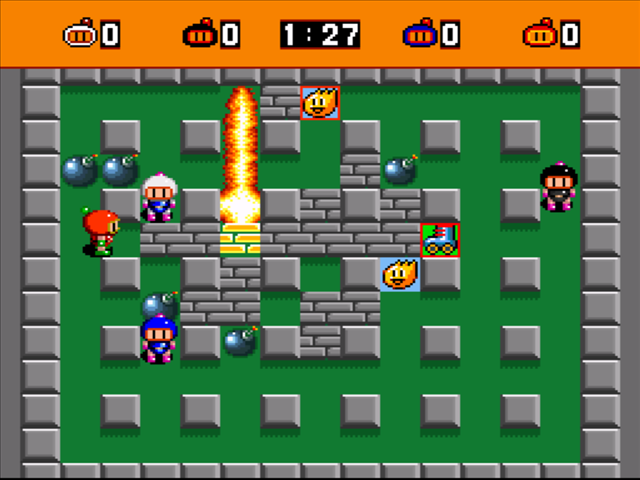
\includegraphics[scale=0.35]{Bilder/bomberman.png}
					\centering
					\caption*{Super Bomberman, SNES \newline Quelle: \url{http://hero.wikia.com/wiki/File:Super-bomberman-1-02.png} }
				\end{figure}
		\end{frame}
		
		\subsection{Musskrit}
		\begin{frame}
			\frametitle{Musskriterien}
				\begin{itemize}
					\item vereinfachte Darstellung
					\item Zweispieler-Modus
					\item Bewegung von Spielfiguren
					\item Platzieren und Explodieren von Bomben
					\item Zerstörung der Blöcke, Gegner
				\end{itemize}
		\end{frame}
	
		\subsection{Wunschkrit}
		\begin{frame}
			\frametitle{Wunschkriterien}
				\begin{itemize}
					\item Sprites
					\item Status-Anzeige
					\item Powerups
					\item mehrere Leben pro Spieler
					\item KI-Gegner
					\item bis zu vier Spieler
					\item Titelbildschirm
				\end{itemize}
		\end{frame}
	
\section{Unser Spiel}
	\subsection{Screenshot}
	\begin{frame}
		\frametitle{Screenshot}
		\begin{figure}[H]
			\centering
			\includegraphics[scale=0.075]{Bilder/Screenshot.png}
			\centering
		\end{figure}
	\end{frame}

	\subsection{Ziele}
	\begin{frame}
		\frametitle{Erfüllte Ziele}
		\begin{itemize}
			\item Zweispieler-Modus
			\item Bewegung von Spielfiguren
			\item Platzieren und Explodieren von Bomben
			\item Zerstörung der Blöcke, Gegner
			\item Kollisionen...später mehr
			\item Sprites
		\end{itemize}
	\end{frame}
	
	
\section{Zeitplan}
	\subsection{Zeitplan}
		\begin{frame}
			\frametitle{Zeitplan}
			\begin{table}[H]
				\centering
				\label{my-label}
				\begin{tabular}{l|l|l}
					Ziel                                      & Zeitvorgabe  & tatsächliche Erfüllung\\
					\hline
					Schaltungsentwurf                         & bis 15.12.17 & 03.12.17\\
					Spielfeld - Layout, Darstellung           & bis 22.12.17 & 07.12.17\\
					Spielfigur - Darstellung, Bewegung        & bis 08.01.18 & 14.12.17\\
					Spielfigur - Kollision                    & bis 15.01.18 & 06.02.18 / z.T. TODO\\
					Bomben - Platzieren, Ticken               & bis 18.01.18 & 21.12.17\\
					Explosionen - Darstellung                 & bis 26.01.18 & 09.01.18\\
					Explosionen - Kollision                   & bis 01.02.18 & 30.01.18\\
					Sprites                                   & - & 01.02.18\\
				\end{tabular}
			\end{table}
		\end{frame}
	
\section{Design}
	\begin{frame}
		\centering \huge Prezi
	\end{frame}
	
\section{Probleme}
	\subsection{Gelöst}
	\begin{frame}
		\frametitle{Gelöste Probleme}
		\begin{itemize}
			\item Fehlerhafte Darstellung der Explosionen
			\begin{itemize}
				\item Spielfeld wird zeilenweise gespeichert
				\item Funktion zum Zeichnen der Explosionen wird durch if-Zweige ausgeführt und erstellt lokale Kopien
			\end{itemize}
			\item Spielfiguren konnten in Blöcke hineinlaufen
			\item Falsche Offset Berechnungen
			\item Sowohl Spielfeld als auch Spielfiguren zeichnen
			\item Sprite-Entities erst asynchron $\implies$ gezeichnet, wenn nicht erlaubt
		\end{itemize}
	\end{frame}
	
	\subsection{Nich gelöst}
	\begin{frame}
		\frametitle{Probleme}
		\begin{itemize}
			\item In der rechten Hälfte funktionieren die Kollisionen nicht mehr
			\item Bei bestimmten Tastendrücken können unzerstörbare Blöcke überlaufen werden
		\end{itemize}
\end{frame}

\section{Demonstration}
	\begin{frame}
		\centering \huge	Showtime!
\end{frame}
		
\end{document}